\documentclass[a4paper]{scrreprt}
 
\usepackage[german]{babel}
\usepackage[utf8]{inputenc}
\usepackage[T1]{fontenc}
\usepackage{ae}
\usepackage{graphicx}
 
\begin{document}
 
\title{Feinentwurf f"ur die Umsetzung des Brettspieles 'Go'}
\author{Harry Flohr (6811837)\\und\\Jan Ole Wellnitz (6796226)}
\maketitle
 
\chapter{Module der Software}
 
\section{Bildverarbeitung (go\_bv.rkt)}
Das Modul Bildverarbeitung ist f"ur das Auslesen des Spielzustandes eines Bildes zust"andig. Ein Bild wird in das Modul geladen und wird dann verarbeitet. Es wird zuerst das Spielbrett aus dem Bild extrahiert und in ein Blauwerte-Bild konvertiert. In diesem Bild wird die Koordinaten des ersten Spielfeldes (oben links) gesucht. An dieser Koordinate wird geschaut, ob die Schwellenwerte f"ur einen wei"sen oder schwarzen Stein getroffen wird. Diese "Uberpr"ufung wird an insgesamt sieben Stellen pro Koordinate vorgenommen. Es wird quadratisch um die Koordinate kontrolliert (siehe Abb. 1.1). Wird ein schwarzer Stein gefunden, wird in die jeweilige Liste der Wert -1 geschrieben. Wird ein wei"ser Stein gefunden, wird der Wert 1 eingetragen. Wird kein Stein gefunden, wird der Wert 0 in die Liste geschrieben.
\begin{figure}[ht]
\centering 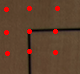
\includegraphics[width=0.3\textwidth]{images/koordinate}
\caption{Suchemuster an Koordinate}
\end{figure}
\\\\
Dieser Prozess wird an jeder Koordinate durchgef"uhrt. Die Koordinaten werden anhand zweier Schrtittweiten (in x - und y-Richtung) ermittelt. Ist das ganze Spielfeld durchkontrolliert, hat das Modul den vollst"andigen Spielstand des Bildes projiziert.

\section{Spielbrett zeichnen (go\_draw\_board.rkt)}
Das Modul Spielbrett zeichnet aus einem Spielstand ein Spielbrett mit dem angegeben Spielstand. Zuerst wird das Grundbrett gezeichnet. Anschlie"send werden die Listen des Spielstandes ausgelesen und die ben"otigten Steine auf das Spielfeld gezeichnet. Die Leserichtung der Listen ist die selbe der Leserichtung beim ermitteln des Spielstandes (von links oben bis rechts unten).

\begin{figure}[ht]
\centering 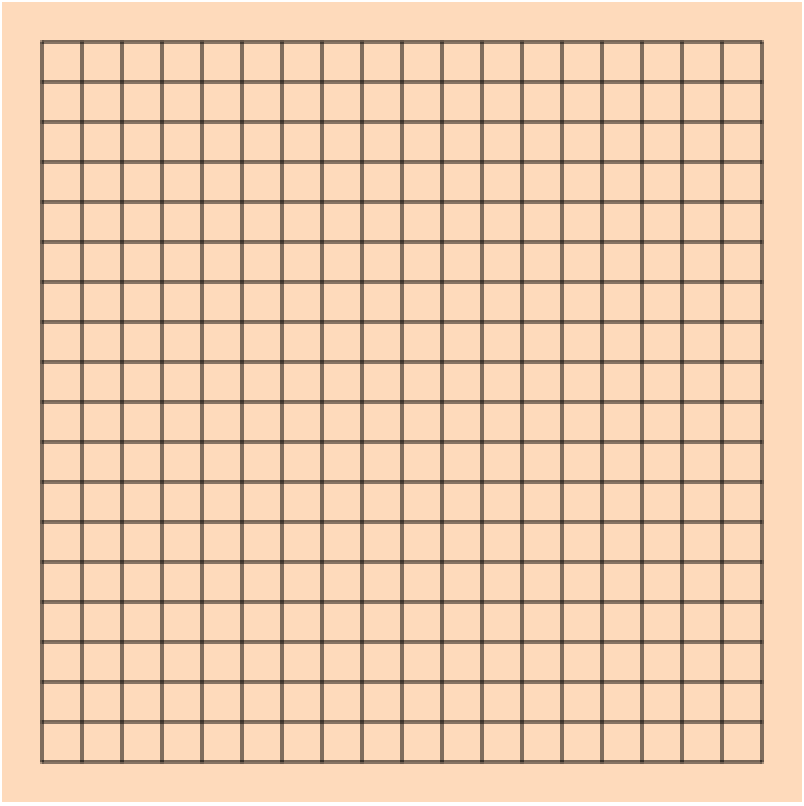
\includegraphics[width=0.3\textwidth]{images/emptyBoard}
\caption{Leeres Spielfeld}
\end{figure}

\begin{figure}[ht]
\centering 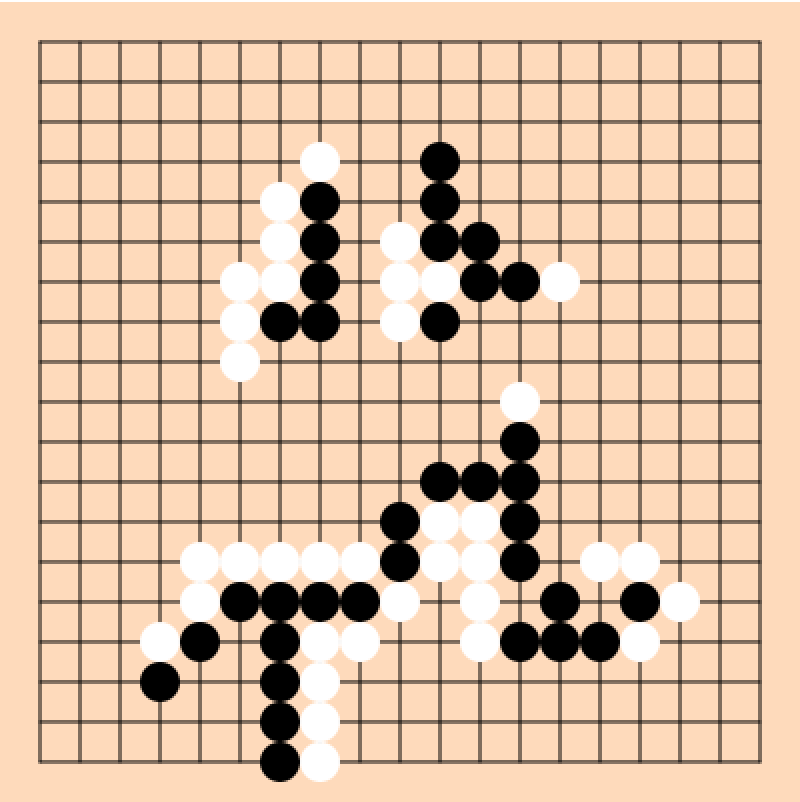
\includegraphics[width=0.3\textwidth]{images/board}
\caption{Belegtes Spielfeld}
\end{figure}

\section{Spielserver (go\_datei.rkt)}
Dieses Modul l"adt aus einer Spielstand-Datei den aktuellen Spielstand.

\section{Spielclient (go\_client.rkt)}
Der Spielclient steuert die Kommunikation des Spielers mit dem Server. Mit dem Spielclient kann  "uber ein Men"u auf drei verschiedene Arten ein Spiel gestartet werden. Es kann ein komplett neues Spiel gestartet werden, es kann ein Spielstand mit einem Bild-Spielstand gestartet werden und es kann ein Spielstand aus einer Datei geladen und gespielt werden. Bei dem Start aus einem Bild-Spielstand muss der Client abfragen, wie viele Steine bereits geschlagen wurden, ob ein Spieler gepasst hat und welcher Spieler am Zug ist. Diese Informationen werden dann zu dem Server geschickt und dieser initialisiert den ersten Spielstand (= World (4.2)). Weiter zeigt der Spielclient w"ahrend eines Spiels den aktuellen Spielstand an und teilt den Spielern mit, ob sie an der Reihe sind, sie einen ung"ultigen Zug vorgenommen haben oder wer gewonnen hat. Der Spieler kann "uber den Client seinen Zug vornehmen und dem Server mitteilen, wo er seinen Stein gesetzt hat. Auch kann er seinen Spielzug passen. Der Spielclient kann w"ahrend des Spiels dem Server mitteilen, dass das aktuelle Spiel in einer Datei gespeichert werden soll.

\section{Spielserver (go\_server.rkt)}
Der Spielserver leitet das Spiel. Zu Beginn erh"alt der Server die Information, ob er ein neues Spiel starten soll oder ein Spiel aus einem Bild oder einer Datei laden soll. Anschlie"send sendet der Server den geladenen Spielstand an die Clients. Er verwaltet den Spielstand (4.2 World) und welcher Spieler am Zug ist. Diese Informationen "ubermittelt der Server immer an die Clients.  Auch pr"uft der Server die "ubermittelten Spielz"uge der Spieler auf ihre G"ultigkeit und teilt den Spielern ggf. mit, dass der Spielzug nicht zul"assig ist. Bei zul"assigen Z"ugen passt der Server den Spielstand (4.2 World) an und "ubermittelt den neuen Spielstand an die Clients. Nach Beendigung eines Spieles, ermittelt der Server den Gewinner und teilt den Spielern (Clients) den Gewinner mit. Erh"alt der Server den Befehl, dass das Spiel gespeichert werden soll, erstellt der Server eine Datei und teilt den Clients mit, dass das Spiel gespeichert wurde.

 \chapter{Schnittstellen}
 \section{Bildverarbeitung}
Das Modul Bildverarbeitung bietet die Schnittstelle, um aus einem Dateipfad eines Bildes einen Spielstand auszulesen. Dies bietet die Funktion '(define (read\_board path))'. An diese Funktion wird der Dateipfad des Bildes "ubergeben und anschlie"send liefert diese den Spielstand der definierten Struktur zur"uck.

\section{Spielbrett zeichnen}
Das Modul zum Zeichnen des Spielbrettes bietet eine Funktion, um ein Spielbrett anhand eines Spielstandes in definierter Struktur zu Zeichnen. Diese Funktion lautet (define (draw\_board\_with\_score game\_score)). An diese Funktion wird der Spielstand "ubergeben und es wird dieser Spielstand gezeichnet zur"uckgeliefert. 

\section{Spielclient}
Ein Spielclient muss in de Lage sein, einen Spielstand (4.2 World) entgegen zu nehmen. Dazu bietes der Client die Schnittstellenfunktion (define (set\_world world)). Diese kann dazu genutzt werden, um den Client einen Spielstand mitzuteilen. Dieser Spielstand wird dann in dem Client dargestellt.

\section{Spielserver}
Der Server bietet eine Reihe an Schnittstellen an.\\
\begin{enumerate}
\item (define (set\_stone posX posY passed)):\\
Der Client kann mit dieser Funktion dem Server mitteilen, an welcher Position er einen Stein setzen m"ochte. Der Server pr"uft die Eingabe und erstellt daraus eine neue World (4.2). Wenn der Spieler gepasst hat, wird ein true f"ur das pass "ubergeben.

\item (define start\_new\_game):\\
Starte ein komplett neue Spiel. Schickt die World an die Clients.

\item (define (start\_game\_pic pic\_path 'stones player player\_Passed)):\\
Starte ein Spiel aus einem Bild heraus. Der Server liest das Bild ein und verarbeitet es mit dem Bildverarbeitungsmodul. Um einen g"ultigen Spielstand zu erstellen, braucht dieser noch die Informationen wie viele Steine bereits geschlagen (Darstellung als Pair '(schwarz . wei"s) wurden, welcher Spieler am Zug ist und ob der vorherige Spieler gepasst hat. Daraus erstellt er einen Spielstand und schickt sie zu den Clients.

\item (define (start\_game\_file file\_path)):\\
Starte ein Spiel aus einem Datei heraus. Der Server liest das Bild ein und verarbeitet es mit dem Dateimodul. Es befinden sich alle n"otigen Informationen in der Datei, sodass keine weiteren Informationen notwendig ist. Schickt anschlie"send die World an die Clients.

\item (define save\_game\_state):\\
Der Server speichert den aktuellen Spielstand in einer Datei und teilt den Spielern das erfolgreiche Speichern mit.
\end{enumerate}

 \chapter{Paketstruktur}

\chapter{Strukturen}

\section{Spielfeld}
Ein Spielfeld besteht aus 19x19 Felder, auf denen Steine positioniert werden k"onnen. Das Spielfeld wird in dem Programm als eine Liste mit 19 weiteren Listen dargestellt. Diese 19 Listen stehen f"ur die y-Koordinaten des Spielfeldes. Jede dieser 19 Listen enth"alt 19 Positionen, um einen Wert einzutragen. Diese Unterlisten stehen f"ur die x-Koordinaten.\\\\
Wenn an einer Position eine 0 steht, befindet sich kein Stein auf dem Spielfeld. Befindet sich dort eine 1, liegt an der Position ein wei"ser Stein. Bei einer -1, liegt an der Position ein schwarzer Stein.\\
\\Darstellung des Spielstandes in Abbildung 1.3:\\\\
'((0 0 0 0 0 0 0 0 0 0 0 0 0 0 0 0 0 0 0)\\
  (0 0 0 0 0 0 0 0 0 0 0 0 0 0 0 0 0 0 0)\\
  (0 0 0 0 0 0 0 0 0 0 0 0 0 0 0 0 0 0 0)\\
  (0 0 0 0 0 0 0 1 0 0 -1 0 0 0 0 0 0 0 0)\\
  (0 0 0 0 0 0 1 -1 0 0 -1 0 0 0 0 0 0 0 0)\\
  (0 0 0 0 0 0 1 -1 0 1 -1 -1 0 0 0 0 0 0 0)\\
  (0 0 0 0 0 1 1 -1 0 1 1 -1 -1 1 0 0 0 0 0)\\
  (0 0 0 0 0 1 -1 -1 0 1 -1 0 0 0 0 0 0 0 0)\\
  (0 0 0 0 0 1 0 0 0 0 0 0 0 0 0 0 0 0 0)\\
  (0 0 0 0 0 0 0 0 0 0 0 0 1 0 0 0 0 0 0)\\
  (0 0 0 0 0 0 0 0 0 0 0 0 -1 0 0 0 0 0 0)\\
  (0 0 0 0 0 0 0 0 0 0 -1 -1 -1 0 0 0 0 0 0)\\
  (0 0 0 0 0 0 0 0 0 -1 1 1 -1 0 0 0 0 0 0)\\
  (0 0 0 0 1 1 1 1 1 -1 1 1 -1 0 1 1 0 0 0)\\
  (0 0 0 0 1 -1 -1 -1 -1 1 0 1 0 -1 0 -1 1 0 0)\\
  (0 0 0 1 -1 0 -1 1 1 0 0 1 -1 -1 -1 1 0 0 0)\\
  (0 0 0 -1 0 0 -1 1 0 0 0 0 0 0 0 0 0 0 0)\\
  (0 0 0 0 0 0 -1 1 0 0 0 0 0 0 0 0 0 0 0)\\
  (0 0 0 0 0 0 -1 1 0 0 0 0 0 0 0 0 0 0 0))\\

\section{World}
Die World setzt sich aus mehreren Informationen zu einer Liste zusammen:

\begin{enumerate}
\item Spielfeld (siehe 4.1)
\item Weltzustand\\
Der Weltzustand gibt an, ob der Client ziehen darf, warten muss oder das Spiel beendet wurde (Zustände: wait, play, lost, won).
\item Geschlagene Steine\\
Die bereits geschlagenen Steine werden als Pair '(schwarz . weiß) übergeben.
\item Gepasster Spielzug\\
Hat der vorherige Spieler in seinem Spielzug gepasst und der Spieler an der Reihe passt ebenfalls, ist das Spiel beendet und die Auswertung startet (Gepasst: true/false). 
\end{enumerate}
Als Beispiel eine mögliche World-Darstellung bei der der aktuelle Spieler am Zug ist, 5 schwarze und 8 weiße Steine geschlagen wurden und der vorherige Spieler nicht gepasst hat. Der Spielstand ist zur Übersicht vereinfacht:
\begin{quotation}
 '(play '(spielfeld) '(5 . 8) false)
\end{quotation}

\end{document}
